%
% ---------------------------------------------------
%
% Proyecto de Final de Carrera:
% Author: Alejandro Hernández Padrón <alu0100703511@ull.edu.es>
% Capítulo: Objetivos 
% Fichero: Cap1_Goals.tex
%
% ----------------------------------------------------
%

% La tecnología de la RA tiene la capacidad de cambiar la forma en la que los estudiantes perciben la realidad física, puesto que permite ampliar el conjunto de información que obtenemos de ella, para facilitar la captación de sus características y elementos.

\chapter{RA en entornos universitarios } \label{chap:RAEntornosUniversitarios}  

En este capítulo trataremos los usos y ventajas de la integración de la realidad aumentada en entornos universitarios.

La realidad aumentada se presenta en el ambito educativo como una tecnología capaz de aportar transformaciones significativas en la forma en que los estudiantes perciben y acceden a la realidad física, proporcionando así, experiencias de aprendizaje más ricas e inmersivas.

En la actualidad en educación, la realidad aumentada rara vez se usa, pero cada vez más docentes, investigadores y desarrolladores están comenzando a moverse hacia nuevos métodos de enseñanza más interactivos. Por ello, con la continua implatación de nuevas tecnologías en las aulas, junto al incremento de dispositivos móviles en la población, sitúa a la RA en una posición destacada para introducirse en las aulas. 


La aplicaciones que tiene la RA, en lo referente a la creación de materiales didácticos y actividades de aprendizaje son múltiples, directas y fáciles de imaginar en prácticamente todas las disciplinas, sobre todo, las relacionadas con las ciencias aplicadas (ingeniería, química y física, biología), pero también en el campo del diseño industrial, la cirugía, la arqueología, etc.
La tecnología de la RA permite cambiar la forma de entender los contenidos de aprendizaje, puesto que aporta nuevas formas de interacción con el mundo real a través de capas digitales de información que amplían, completan y transforman en cierto modo la información inicial.


Los beneficios potenciales de la RA aplicados a la educación incluyen:
\begin{itemize}

    \item Aumentar o enriquecer la información de la realidad para hacerla más comprensible al estudiante.
    
    % \item Permite múltiples formas de visualización de conceptos teóricos difíciles.

    \item El uso de una interfaz tangible para la manipulación de objetos, que permite observar un objeto desde diferentes puntos de vista,
    seleccionando, el estudiante, el momento y posición de observación.

    \item Potenciar el aprendizaje ubicuo \cite{URL::AprendizajeUbicuo}.
    
    \item Crear escenarios “artificiales” seguros para los estudiantes
    como pueden ser laboratorios o simuladores. 

    \item Enriquecer los materiales impresos para los estudiantes con información adicional en diferentes soportes.
    
    \item Facilita la colaboración efectiva y discusión entre los estudiantes.
    \item 
    Furthermore, AR applications can enhance the learning process, learning motivation and effectiveness
\end{itemize}

Numerosos articulos han demostrado la eficacia de que las aplicaciones de RA pueden mejorar el proceso de aprendizaje, aumentar la motivación y la efectividad \cite{URL::animationeco} \cite{URL::ar2}. Pero hay que tener en cuenta una serie de requisitos a la hora de diseñar un sistema educativo de RA para que el estudiante no se distraiga con su uso y asegurar que el objetivo de mejorar el aprendizaje se cumpla. Estos requisitos son:

\begin{itemize}
    \item Ser sencillo y robusto.
    \item Permitir que el educador ingrese información de manera simple y efectiva.
    \item Proporcionar al alumno información clara y concisa.
    \item Permitir una fácil interacción entre estudiantes y educadores.
    \item Realizar procedimientos complejos transparentes para los alumnos.
    \item Ser rentable y fácilmente extensible.
\end{itemize}


\section{Aplicaciones en entornos universitarios}

\subsubsection{Prácticas en laboratorios} 
En las realizacines de las prácticas en un laboratorio, existe una gran gama de herramientas y máquinas que son desconocidas para el estudiante. Para facilitar el uso de este instrumental, la RA permite asociar a cada elemento del laboratorio, información sobre el mismo, tutoriales de uso, indicaciones de los pasos a seguir para la elaboración de la práctica. Esto permite agilar el proceso de realización de las prácticas evitando que el alumno requiera del profesor para resolver parte de sus dudas y permitiendole centrarse más en la realización de la práctica.

\subsubsection{Practicas de campo y visitas} 

La posibilidad de realizar una visitar un museo e identificar cada estatua o cuadro, y mostrar información adicional sobre su autor, datos historicos de las obras, reconoer estilos e influencias del autor para su realización, permite al usuario mejorar su adquisición de conocimiento al mezclarse el objeto de conocimiento y conocimiento en el mismo lugar. Este mismo concepto se puede aplicar a prácticas de campo a medios rurales, bosques, montañas y lagos, permitiendo al usuario identificar la flora y la fauna del terreno y mostrar características únicas sobre ellos, que a simple vista son imperceptibles.

\subsubsection{Libros}
A los libros electrónicos o en formato papel se añade realidad aumentada utilizando como activador de la información los textos, ilustraciones, encabezados, pies de página, etc., y como información adicional en muchos casos se incluye la biografía del autor, los pies de página, vídeos que desarrollan la acción más ampliada, textos adicionales y audios. Se denominan libros aumentados.
o El libro enmarcado en el proyecto: “HUSSO DIGITAL: LA CIUDAD UNIVERSITARIA EN REALIDAD AUMENTADA, “El libro aumentado de Eduardo Torroja” es un claro ejemplo.

    
\subsubsection{Información sobre la universidad}  

Dentro de sus aplicaciones a los centros de universidad encontramos el uso de marcadores por el que el alumno pueda identificar edificios y centros para guiarlos hasta el aula en la que tiene la próxima clase. Tambien se podría utilizar para mostrar información sobre eventos, seminarios o jornadas, y poder apuntarse a los mismos con simplemente escanear un código QR.

% \subsubsection{Aprendizajes experimentales} 

% prácticamente todas las disciplinas tienen una parte experimental que pueden realizarse con realidad aumentada facilitando en gran medida el aprendizaje y el desarrollo de destrezas transversales. Ejemplos claros pueden ser en medicina, donde el uso de las google glass de forma experimental hace un par de años fue muy mediático, en arquitectura e ingenierías, la posibilidad de realizar y ver modelos en 3D de diferentes edificios y construcciones es muy útil en el aprendizaje del alumno. En química o física con aplicaciones como las que aparece en el bloque 3 dedicado a programas y aplicaciones, también en ramas como la Gabinete de Tele-Educación 24 Universidad Politécnica de Madrid Realidad Aumentada en Educación biología, arte, historia, diseño, idiomas, geografía, matemáticas, urbanismo, música, geometría, etc.


\section{Ejemplos de uso de la RA}

\subsubsection{Fabricación de un automóvil de carreras} 

Los estudiantes de la Universidad de Bath están utilizando una nueva herramienta RA desarrollada por la compañía de tecnología Rocketmakers. La herramienta RA ayudará con la construcción de la carcasa del automóvil, conocida como monocasco, específicamente con la aplicación de laminados de fibra de carbono. Su vehículo competirá en la competencia de Fórmula Estudiantil 2019 organizada por la Institución de Ingenieros Mecánicos.

Este proceso se llevará a cabo durante una semana, y los estudiantes de Team Bath Racing trabajarán por turnos para aplicar cada laminado de fibra de carbono precortado en la ubicación correcta. La herramienta de Rocketmakers crea una versión RA del monocasco con la forma, ubicación y orientación correctas de cada segmento de laminado visible para el usuario durante el proceso de aplicación. Para ello utilizarán las Microsoft Hololens \cite{URL::hololens}, con archivos de diseño asistido por computadora (CAD) que los estudiantes han desarrollado.

\begin{figure}[h]
    \centering
    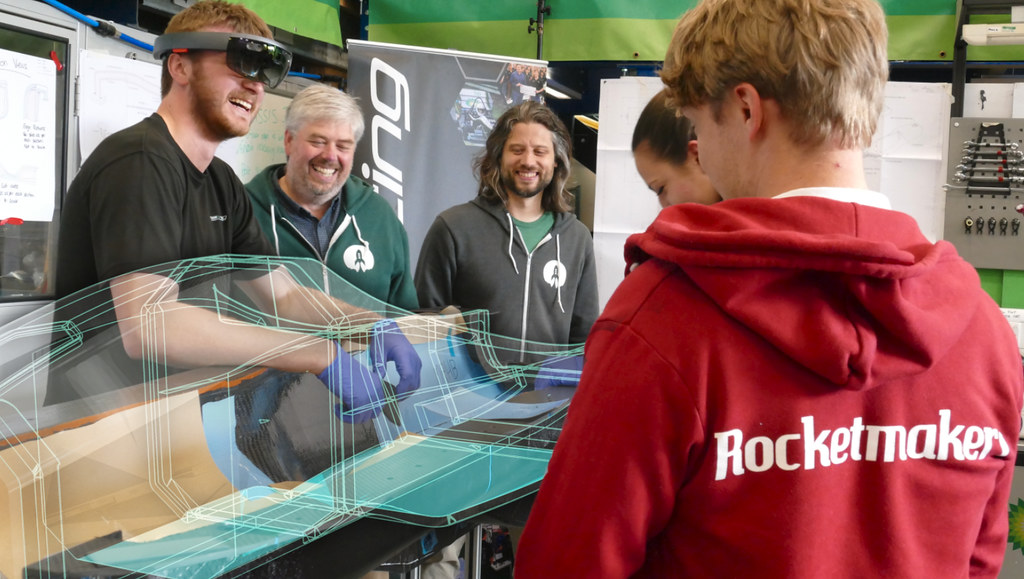
\includegraphics[width=0.6\linewidth]{carAR}
    \caption{Construcción de un automóvil de carreras gracias a la RA.}
    \label{fig:xyz}
\end{figure}    
 

\subsubsection{AR Sandbox} 
AR Sandbox \cite{URL::sandbox} es el resultado de un proyecto desarrollado por W.M. El Centro Keck para la Visualización Activa en las Ciencias de la Tierra (KeckCAVES), junto con el Centro de Investigación Ambiental UC Davis Tahoe, Lawrence Hall of Science y ECHO Lake Aquarium and Science Center.

El proyecto combina aplicaciones de visualización 3D con una exhibición de sandbox para enseñar conceptos de ciencias de la tierra. La caja de arena de realidad aumentada  permite a los usuarios crear modelos de topografía al dar forma a la arena real, que luego se aumenta en tiempo real mediante un mapa de color de elevación, líneas de contorno topográficas y agua simulada. El sistema enseña conceptos geográficos, geológicos e hidrológicos, como la forma de leer un mapa topográfico, el significado de las curvas de nivel, las cuencas hidrográficas, los diques, etc.

\begin{figure}[h]
    \centering
    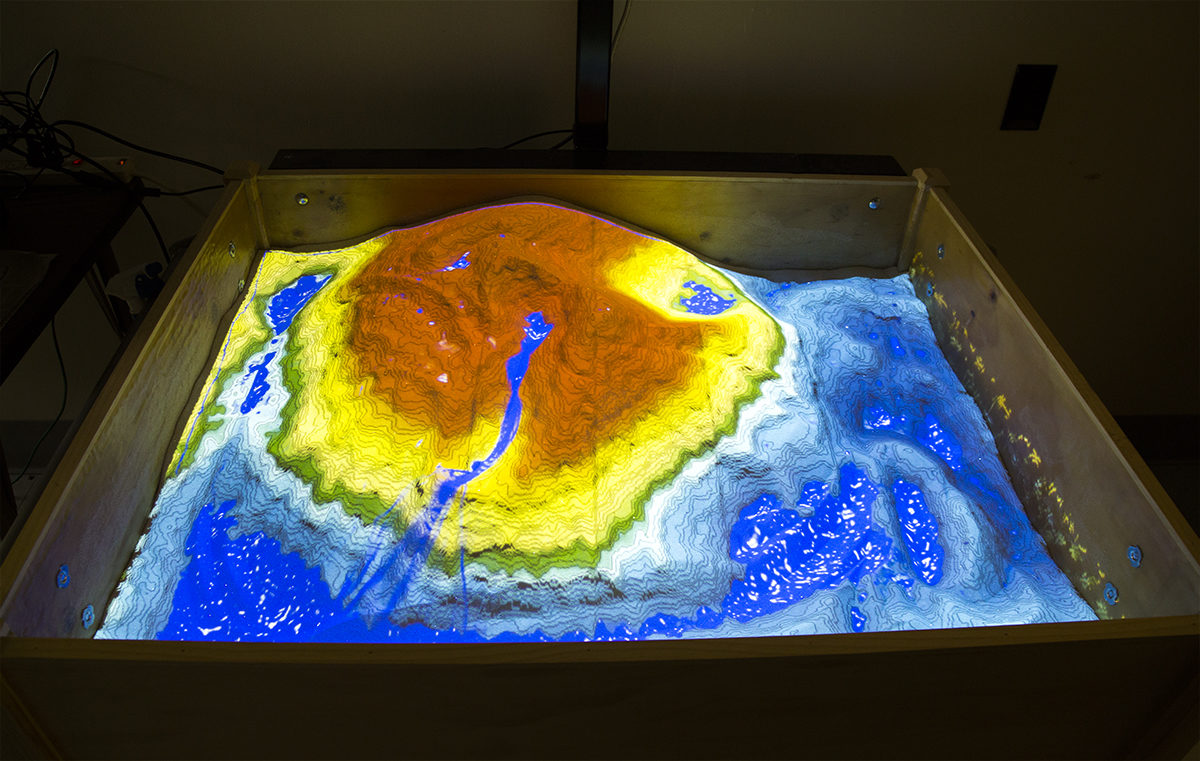
\includegraphics[width=0.8\linewidth]{sandAR}
    \caption{Funcionamiento de AR Sandbox.}
    \label{fig:xyz}
\end{figure}    



% Varios científicos de la Universidad Carlos III de Madrid han diseñado unas gafas inteligentes que permiten conectar a profesores y alumnos en tiempo real en el aula. Telmo Zarraonandia, Ignacio Aedo, Paloma Díaz y Álvaro Montero a través del artículo, An augmented lecture feedback system to support learner and teacher communication explican su funcionamiento. Con tan solo ponerse las gafas en cuestión, el docente obtendrá información del alumno al mirar tras ellas. Notas y comentarios que lanzarán los alumnos al docente los podrá recibir con tan solo observar a su grupo de clase.

% El feedback estará asegurado en estas aulas, de nuevo utilizando como recurso tecnológico la realidad aumentada.

% % https://e-archivo.uc3m.es/bitstream/handle/10016/17136/augmented_british_2013_pp.pdf?sequence=1&isAllowed=y

% https://www.itv.com/news/2019-05-09/students-use-augmented-reality-tool-to-help-manufacture-race-car/

% Collaborative work of students within the
% Augmented Reality application Construct3D

% Libros de texto aumentados 



% Modelos 3D utilizados en arquitectura para la visualización de dispositivos




